\subsection{Точки Лагранжа}

\textbf{Точки Лагранжа} --- точки в системе из двух массивных тел, в которых третье тело с пренебрежимо малой массой, не испытывающее воздействие никаких других сил, кроме гравитационных, со стороны двух первых тел, может оставаться неподвижным относительно этих тел (Рис.13).

Точки $L_1$, $L_2$ и $L_3$ лежат на одной прямой, соединяющей два массивных тела. Точки $L_4$ и $L_5$ образуют равносторнние треугольники с массивными телами.

Приближённые формулы для вычислений расстояний до $L_1$, $L_2$ и $L_3$ от центра масс:
$$r_1=R\left(1-\sqrt[3]{\frac{\alpha}{3}}\right); r_2=R\left(1+\sqrt[3]{\frac{\alpha}{3}}\right); r_3=\left(1+\frac{5}{12}\alpha\right)$$
Где $\alpha=M_1/(M_2+M_3)$, $R$ --- расстояние между телами, $M_1$ --- масса более массивного тела, $M_2$ --- масса второго тела.

Если $M_2\ll M_1$, то точки $L_1$ и $L_2$ находятся примерно на равном расстоянии от тела $M_2$. Примерное значение этого расстояния можно вычислить по формуле:
$$r\approx R\sqrt[3]{\frac{M_2}{3M_1}}$$
\begin{center}
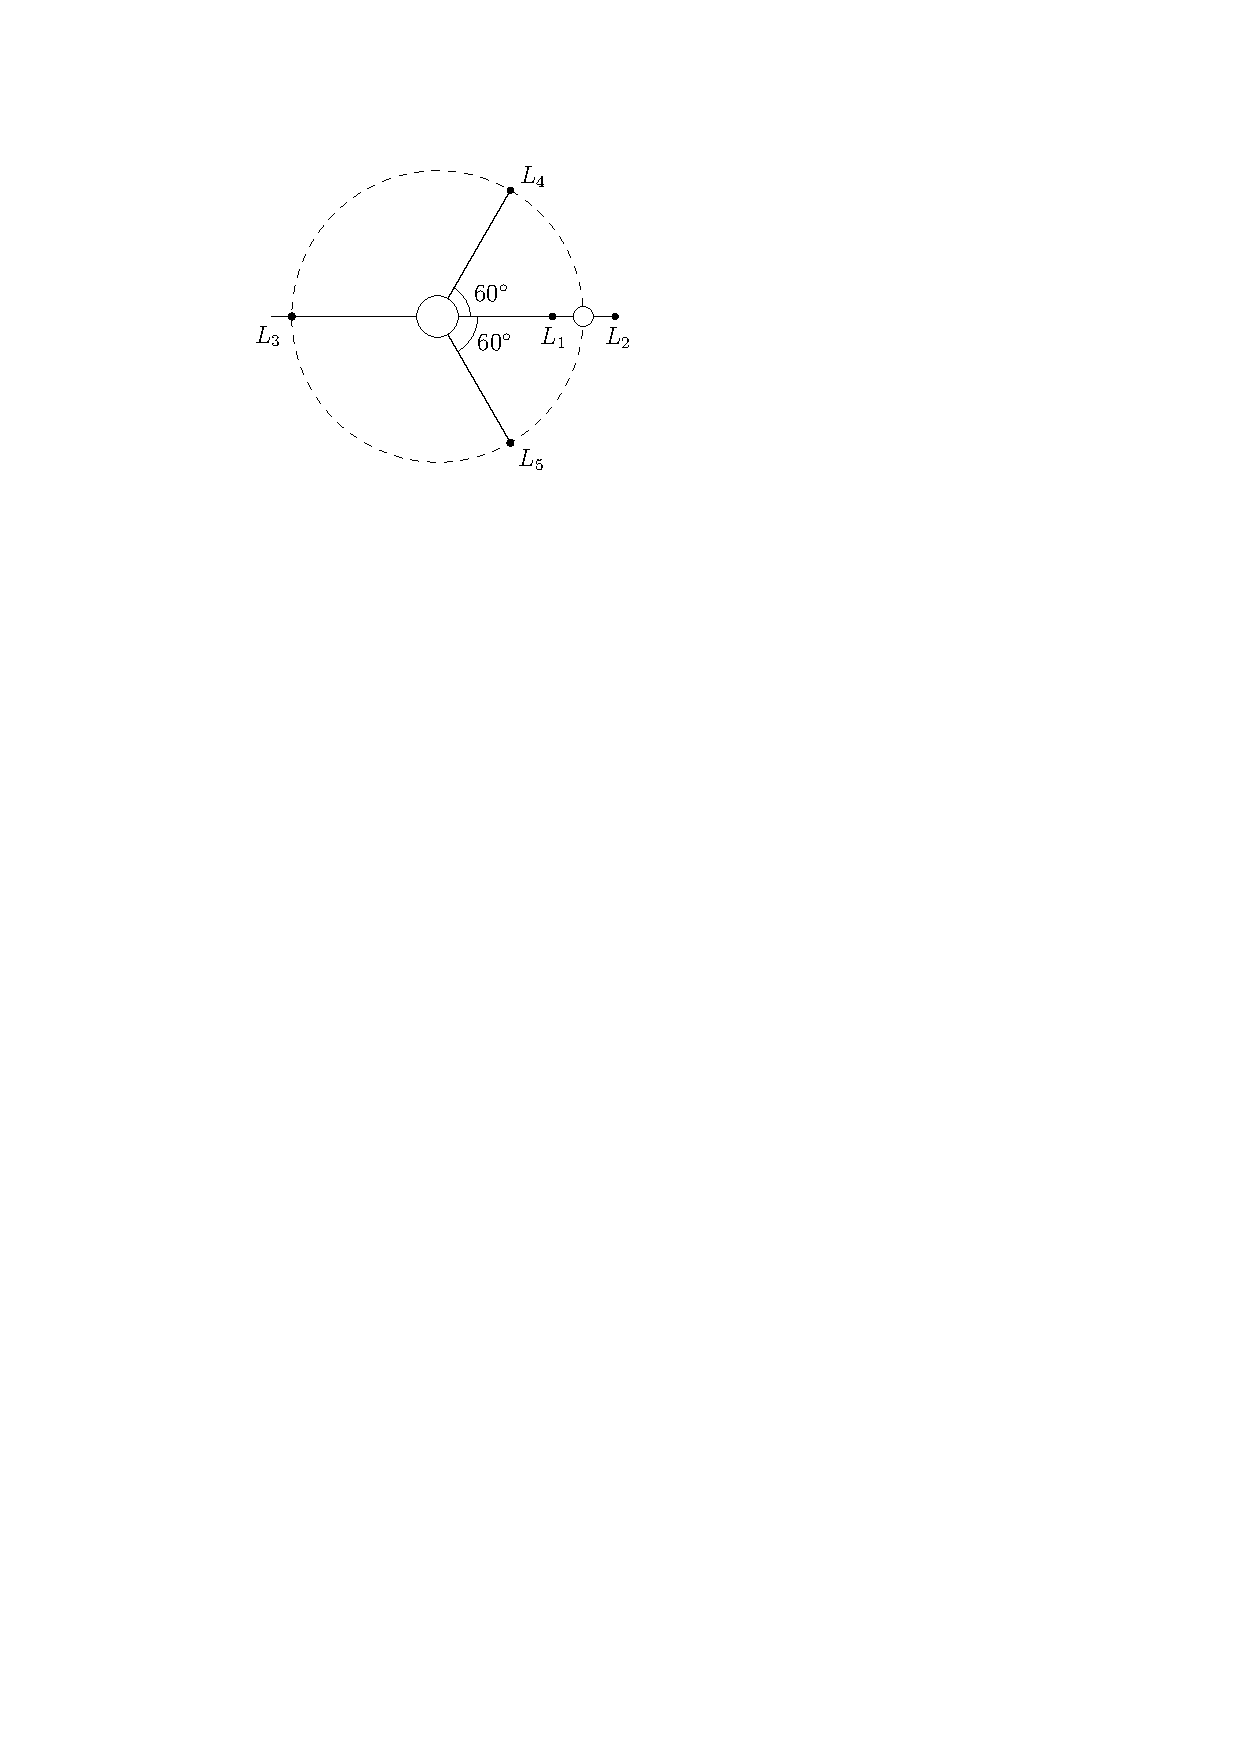
\includegraphics[width = 0.45\textwidth]{Lagrange's_points}
\begin{figure}[h!]
\caption{Точки Лагранжа}
\end{figure}
\end{center}